\begin{figure*}\centering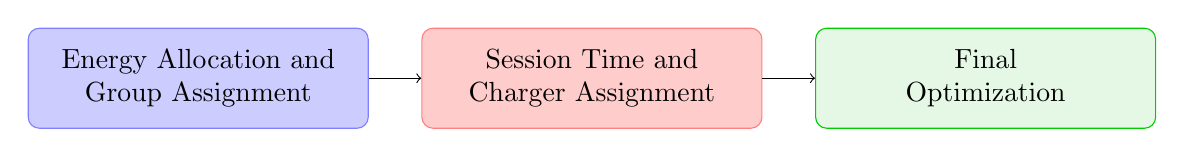
\begin{tikzpicture}
	\node[rectangle, draw=blue!50, fill=blue!20, minimum width=1.7in, minimum height=0.5in, rounded corners](set1) at (0,0) {\begin{tabular}{c} Energy Allocation and\\ Group Assignment\end{tabular}}; 
	\node[rectangle, draw=red!50, fill=red!20, minimum width=1.7in, minimum height=0.5in, rounded corners](set2) at (5,0) {\begin{tabular}{c} Session Time and \\Charger Assignment \end{tabular}}; 
	\node[rectangle, draw=green!80!black, fill=green!70!black!10, minimum width=1.7in, minimum height=0.5in, rounded corners](set3) at (10,0) {\begin{tabular}{c} Final \\ Optimization\end{tabular}}; 
	\draw[->] (set1.east) -- (set2.west);
	\draw[->] (set2.east) -- (set3.west);
\end{tikzpicture}\caption{Overall Processing Chain}\label{fig:processChain}\end{figure*}

